% Template for a Computer Science Tripos Part II project dissertation
\documentclass[12pt,a4paper,twoside,openright]{report}
\usepackage[UKenglish]{isodate}
\usepackage[pdfborder={0 0 0}]{hyperref}    % turns references into hyperlinks
\usepackage[margin=25mm]{geometry}  % adjusts page layout
\usepackage{graphicx}  % allows inclusion of PDF, PNG and JPG images
\usepackage{parskip}
\usepackage{verbatim}
\usepackage{color}
\usepackage{enumitem}
\usepackage{longtable}
\usepackage{microtype}
\usepackage{stmaryrd}
\usepackage{amsmath}
\usepackage{amssymb}
\usepackage{lilyglyphs}
\usepackage{fontspec}
\usepackage{csquotes}
\usepackage{float} % figure positioning

% pseudocode typesetting
\usepackage{algorithmicx}
\usepackage[noend]{algpseudocode}
\usepackage{algorithm}

\newcommand{\set}[1]{ \left\{ #1 \right\} }
\newcommand{\insharp}[0]{\sharp[raise=0.1,scale=0.8]}
\newcommand{\inflat}[0]{\flat[raise=0.1,scale=0.8]}

\usepackage[style=numeric,backend=biber]{biblatex}
\addbibresource{refs.bib}

\usepackage{docmute}   % only needed to allow inclusion of proposal.tex

\newcommand{\todo}{\textcolor{red}{\textbf{todo}~}}

\raggedbottom                           % try to avoid widows and orphans
\sloppy
\clubpenalty1000%
\widowpenalty1000%

\renewcommand{\baselinestretch}{1.1}    % adjust line spacing to make
                                        % more readable

\begin{document}

\cleanlookdateon

%%%%%%%%%%%%%%%%%%%%%%%%%%%%%%%%%%%%%%%%%%%%%%%%%%%%%%%%%%%%%%%%%%%%%%%%
% Title

\pagestyle{empty}

\rightline{\LARGE \textbf{Alex Coplan}}

\vspace*{60mm}
\begin{center}
\Huge
\textbf{A Comparison of Statistical Models and Recurrent Neural Networks for the
Generation of Music} \\[5mm]
Computer Science Tripos -- Part II \\[5mm]
St Catharine's College \\[5mm]
\today  % today's date
\end{center}

%%%%%%%%%%%%%%%%%%%%%%%%%%%%%%%%%%%%%%%%%%%%%%%%%%%%%%%%%%%%%%%%%%%%%%%%%%%%%%
% Proforma, table of contents and list of figures

\pagestyle{plain}

\chapter*{Proforma}

{\large
\begin{tabular}{r p{10.5cm}}
Name:               & \bf Alex Coplan                       \\
College:            & \bf St Catharine's College                     \\
Project Title:      & \bf A Comparison of Statistical Models and Recurrent
Neural Networks for the \newline Generation of Music \\
Examination:        & \bf Computer Science Tripos -- Part II, July 2017  \\
Word Count:         & \todo\footnote{1} \\
Project Originator: & Alex Coplan \\
Supervisor:         & Matthew Ireland                    \\ 
\end{tabular}
}
\footnotetext[1]{This word count was computed
by \texttt{detex diss.tex | tr -cd '0-9A-Za-z $\tt\backslash$n' | wc -w}
}
\stepcounter{footnote}


\section*{Original Aims of the Project}

The original aim of this project was to implement two models for music
generation and subsequently compare them: namely, a \emph{recurrent neural
network} and \emph{multiple viewpoint system}. The two models were
to be compared using both a listening survey involving human participants and
objective metrics of evaluation, such as information-theoretic measures
of predictive performance.

\section*{Work Completed}

All that has been completed appears in this dissertation.

\section*{Special Difficulties}

\todo
 
\newpage
\section*{Declaration}

I, Alex Coplan of St Catharine's College, being a candidate for Part II of the
Computer Science Tripos, hereby declare that this dissertation and the work
described in it are my own work, unaided except as may be specified below, and
that the dissertation does not contain material that has already been used to
any substantial extent for a comparable purpose.

\bigskip
\leftline{Signed }

\medskip
\leftline{Date }

\tableofcontents

\listoffigures

\newpage
\section*{Acknowledgements}

Acknowledge acknowledge acknowledge.

%%%%%%%%%%%%%%%%%%%%%%%%%%%%%%%%%%%%%%%%%%%%%%%%%%%%%%%%%%%%%%%%%%%%%%%
% now for the chapters

\pagestyle{headings}

\chapter{Introduction}

The modelling and automated generation of music is a central task in an approach
to understanding computational creativity. It is natural to ask whether
computers can produce music that is compelling to humans, and indeed, this
question has long been posed by researchers, with practical efforts dating back
to the mid-1950s \cite{ames1987automated}. 

The aim of this work is to implement and compare two modern techniques for
\emph{melody generation}, a task highly amenable to statistical modelling and
machine learning. 

An automated system for melody generation is motivated by end-user applications
in \emph{computer-assisted composition}, whereby the system can provide
inspiration for a human composer, either by generating entirely novel melodies
within stylistic constraints, or extemporising on or extending melodic
fragments written by the human composer. Such a system might augment the
capabilities of typical music notation software. 

Markov modelling is a simple yet effective technique for capturing the
statistics of sequential data. An obvious tool to apply to the modelling of
melody is the Markov chain \cite{ames1989markov}. However, an important
observation to make is that music has a rich underlying structure: modelling the
statistics of notes directly (the \emph{surface structure}) is insufficient to
capture the complex language of musical style. This observation motivated the
development of more sophisticated models, known as \emph{multiple viewpoint
systems} \cite{conklin1995viewpoints}.  A multiple viewpoint system exploits the
rich underlying event structure of complex languages by combining the
predictions of an ensemble of context models, each modelling a different
attribute of the event space.

Recurrent neural networks (RNNs), the natural topology of neural network for
modelling sequential data, have been widely applied to tasks such as language
modelling \cite{graves2013generating}, machine translation
\cite{sutskever2014sequence}, and indeed to the modelling of music
\cite{liang2016bachbot}. A RNN is an end-to-end sequence learning tool which
relies on very little domain knowledge aside from the chosen input
representation. This means that a system designed for character-level language
modelling can equally be trained to model melody without changing the network
architecture. In practice, however, we shall see that slight architectural
modifications can be beneficial.

In this work, we compare the performance of multiple viewpoint systems with that
of recurrent neural networks on a task of stylistically-constrained melody
generation. In particular, we assess predictive performance, in terms of a
\emph{cross-entropy} loss function, on a corpus of melodies used in the chorale
harmonisations of J.S.\ Bach. Furthermore, we compare the sampled outputs from
each model by means of a listening survey involving human participants.

A high-level goal of this work which motivates the choice of models involved is
understanding to what extent \emph{feature engineering} impacts the
effectiveness of musical models. A recurrent neural network, at one extreme, is
a domain-independent, end-to-end learning system, capable of learning to extract
high-level features from sequential data \cite{Goodfellow-et-al-2016}. A system
of viewpoints, however, relies on its creator to use domain knowledge to
determine a set of salient features, encoded in the form of the \emph{pool} of
viewpoints made available to the system.

\section{Background}

\subsection{Music Theory}

The development and implementation of the recurrent neural network in this work
can be understood with minimal knowledge of music theory. In general, the
multiple viewpoint formalism can also be expressed independently of any domain
knowledge.  However, to understand the application of the multiple viewpoint
framework to music requires an elementary understanding of music theory.  This
section introduces the relevant terminology to enable such discussion.

We shall constrain our discussion to the context of Western classical music,
since the style which we wish to model lies within this context. A \emph{pitch}
is an abstract concept which is related to the frequency of a musical note.
Formally, if $p,q$ are pitches with corresponding frequencies $\nu_p,\nu_q$,
then if $\nu_q = 2\nu_p$, $p$ and $q$ are said to span an \emph{octave}, with
$q$ an octave above $p$. In Western classical music, each octave is divided into
twelve distinct \emph{note names} (A through G modified by accidentals
\insharp{} or \inflat{}). A note name, such as `B\inflat' (or, equivalently,
A\insharp), is typically thought of as not just a single pitch, but a
\emph{pitch class}, the set of all pitches an integer number of octaves above or
below any pitch with that note name.  Formally, given some reference frequency
$\nu_n$ for a note name $n$, the set of frequencies of the pitches in the pitch
class for $n$ is given by $\set{ 2^k \cdot \nu_n\ |\ k \in \mathbb{Z} }.$

The mapping between pitch and frequency is known as \emph{temperament}, which on
modern instruments is typically \emph{equal}, meaning that the frequency space is
equally divided among the twelve pitches in an octave. More precisely, the
$(k+1)$\textsuperscript{th} note of the chromatic scale with base frequency $\nu_0$ is
given by $2^{k/12}\cdot\nu_0$. As an aside, all recordings of
model outputs in this work were made using equal temperament. Herein
we will work with the abstraction of pitch, ignoring the underlying frequencies
of notes.

To refer to specific pitches, we make use of \emph{scientific pitch notation}
(SPN). Write $N_k$ where $N$ is a note name and $k$ is an octave number. To
ground all the definitions made thus far, we use the standard reference
frequency $\mathrm{A}_4 \triangleq 440\ \mathrm{Hz}$. An \emph{interval} refers
to the difference in pitch between two notes. Consecutive note names are said to
be a \emph{semi-tone} apart, and an interval of two semi-tones is known as a
\emph{tone}. Later in this work we shall further abstract pitch and intervals
using MIDI pitch numbering, and further concepts shall be defined as necessary.
In the MIDI tuning standard, $\mathrm{A}_4$ corresponds to pitch number $69$.

\todo talk about key/tonality? this section getting quite long \ldots

\subsection{Melody Generation}

\todo Reference literature to explain why this is difficult task. Background in
Pearce's thesis?

\section{Work Accomplished}

A complete framework for implementing Multiple Viewpoint Systems in \verb!C++!
has been implemented. The formalism as described by Conklin et al.\
\cite{conklin1995viewpoints} has been fully implemented.  At the core of the
framework, the \emph{prediction by partial match} (PPM) algorithm
\cite{cleary1984ppm} was implemented for smoothing variable-order context
models, which can be parameterised over arbitrary types using \verb!C++!
templates. The distributions predicted by these context models can be combined
using either a \emph{weighted arithmetic} scheme (as per
\cite{conklin1995viewpoints}) or \emph{weighted geometric} scheme, the latter
found to be more effective by both Pearce \cite{pearce2005construction} and
Whorley \cite{whorley2013phd}.

Abstractions were made such that, using these primitives, \emph{primitive},
\emph{derived}, \emph{linked}, and \emph{triply-linked} viewpoints can be
instantiated over arbitrary combinations of types. Both a \emph{long-term}
model, for capturing regularity throughout the corpus, and a \emph{short-term}
model, for capturing the regularity within a composition, were implemented.
Sampling by random walk was implemented for melody generation.  Finally, an
automatic viewpoint selection algorithm in the form of \emph{forward step-wise
selection} \cite{whorley2013phd} was implemented.

Code for corpus preparation and analysis was written in Python using the
\texttt{music21} package. This code was used by both the MVS and RNN
implementations.

A multi-layer LSTM recurrent neural network was implemented in Python using
TensorFlow \cite{abadi2016tensorflow}. The network includes \emph{dropout} for
regularisation as per Zaremba et al.\ \cite{zaremba2014recurrent}. A decoupled
``front-end'' to the RNN was implemented which allows the same internal model to
be used for character-level language modelling and music modelling. Random walk
sampling was implemented for generation. In addition, modifications to the
conventional sequence-prediction RNN architecture were made by feeding the
network additional \emph{global} musical information at each timestep, which was
found to improve performance significantly.

Finally, a website for human evaluation was developed. This will be discussed in
detail in Chapter~\ref{chap:eval}.

\section{Related Work}

\subsection{Multiple Viewpoints}

The general method of multiple viewpoints was first applied to music in 1986 by
Ebcioğlu in a rule-based system for chorale harmonisation
\cite{ebcioglu1986expert}.  This system used hand-crafted rules written in
first-order logic which were expressed in terms of different viewpoints of the
music. This system did not make use of Markov models, the main primitive
underlying \emph{statistical} viewpoint systems.

In 1988, Conklin and Cleary \cite{conklin1988modelling} applied multiple
viewpoints with underlying probabilistic Markov models to modelling Gregorian
chant and simple two-part polyphony. The authors make use of the
\emph{prediction by partial match} (PPM) algorithm \cite{cleary1984ppm} for
smoothing variable-order Markov models, but the escape method used is not
specified.  An ad-hoc, unweighted method is used for combining the predictions
of viewpoints.

Conklin and Witten went on to develop a formalism around multiple viewpoints in
a key 1995 paper \cite{conklin1995viewpoints}. The authors justify discounting
the
\emph{knowledge engineering} approach:

\begin{displayquote}
``There are too many exceptions to any
logical system of musical description, and it will be difficult to ensure the
completeness of an intuited theory. The system will always exclude some valid
pieces. The generations of a theory are bound to reflect the biases of an
engineer; this is the only way they might be called creative.''
\end{displayquote}

With similar reasoning, we shall only consider models which learn from data.  At
this point in time, the convention in the literature became to use ``multiple
viewpoint system'' to refer to \emph{statistical} viewpoint systems with
underlying context models: a convention we shall also adopt.

Many of the ideas in this paper were first published in Conklin's 1990 thesis
\cite{conklin1990prediction}. The notion of separate \emph{long-term} and
\emph{short-term} models in a viewpoint system was introduced in this work.
Conklin also details a principled method for distribution combination, namely
\emph{entropy-weighted arithmetic combination}. 

Among the contributions from his 2005 thesis \cite{pearce2005construction},
Pearce introduces a \emph{geometric} viewpoint combination technique, shown to
outperform its arithmetic counterpart, as well as a method for automatic
viewpoint selection, thereby greatly reducing the selection bias in multiple
viewpoint systems. The work concerns the modelling of melody.

More recent work by Whorley~\cite{whorley2013phd} uses multiple viewpoint
systems to model four-part harmony in Bach chorales.

\subsection{Recurrent Neural Networks}

\todo Pre-LSTM applications to music, invention of LSTM, then post-LSTM
applications to music.

\section{Structure}

\todo

\chapter{Preparation}

\todo mention \textbf{starting point} here.

\section{Deliverables}

Recalling the proposal, the success criteria for the project include the
following deliverables:
\begin{itemize}
  \item A program or tool for importing the corpus in the desired format.
  \item A multiple viewpoint system (MVS) capable of generating melody.
  \item A recurrent neural network (RNN) capable of generating melody.
  \item Quantitative and human evaluation.
\end{itemize}

This chapter concerns the ideas behind the first three of these, along with
a discussion of the research and decisions made prior to implementation.
Chapter~\ref{chap:eval} will discuss the design and implementation of the
human evaluation survey in detail, as well as quantitative evaluation.

\section{Corpus Preparation}

The chosen corpus was a set of chorale melodies used in the harmonisations of
J.S.\ Bach. The Bach Chorales are a corpus of great interest in the
computational modelling of music: the style is unified, yet with significant
inter-opus variance; it is not too complex, yet not overly simplistic.

Initial inspection of relevant corpora and their formats indicated that writing
a parser for an established music notation format such as MusicXML would take a
considerable amount of time and offer limited flexibility. After further
research, it was decided that the Python package \texttt{music21} would be
utilised. \texttt{music21} is an open-source toolkit for computational
musicology. This package was especially useful for the task of corpus
preparation due to the following features:
\begin{itemize}
  \item Built-in corpora including the Bach chorales in MusicXML format.
  \item Parser for various music notation formats, including MusicXML.
  \item High-level features for manipulating musical data.
\end{itemize}

As will be discussed later, the flexibility offered by \texttt{music21} became
of great use later in the project as the requirements in corpus preparation and
analysis changed.

An internal format for melody based on a representation used commonly in the
multiple viewpoint system literature (e.g.\ \cite{conklin1995viewpoints}) was
decided on. It was decided that musical time should be quantised with a quantum
of $1/16$\textsuperscript{th} notes (semiquavers). 

This representation was to be used internally for both the MVS and
RNN implementations. A note $n$ is represented as a tuple $(p,o,d) \in
\mathbb{N}^3$ where $p$ is the MIDI pitch number of $n$, $o$ is the onset 
time, and $d$ is the duration. A melody is then a list of such tuples. Note that
rests are not explicitly represented in this encoding.

\section{Multiple Viewpoint Systems}

In this section, the key theory, algorithms, and data structures underpinning
multiple viewpoint systems are introduced. The notation and formalism is as per
Conklin and Witten \cite{conklin1995viewpoints}. We start by defining some
notation which will be used throughout this section.

\begin{itemize}[itemsep=0mm]
  \item If $\tau$ is a type, then $[\tau]$ is the \emph{syntactic domain} of
    that type: all elements of type $\tau$.   
  \item $S^*$ denotes the set of all sequences drawn from a set $S$.
  \item $e_i^j$ abbreviates the sequence $(e_i,e_{i+1},\ldots,e_{j-1},e_j)$ and
    $()$ the empty sequence.
  \item $s :: e$ denotes the sequence $s$ with event $e$ appended.
  \item $\zeta$ denotes the \emph{event space}, the set of all possible events
    that can occur in sequences of interest. For example, a very simple event
    space for melody might be:
    $$ [\mathrm{pitch}] \times [\mathrm{duration}] \times [\mathrm{onset}]. $$
\end{itemize}

\subsection{Context Models}

The central primitive underlying a multiple viewpoint system is the
\emph{context model}. In general, a context model over some type $\tau$ is
a data structure storing sequences in $[\tau]^*$, together with an inference
procedure predicting distributions over $[\tau]$.

While first-order Markov chains make predictions based on just one timestep of
context, an $n$\textsuperscript{th} order Markov chain makes predictions based
on $n$ elements of context. For notational convenience, and for consistency with
the literature, we generally refer to the \emph{history} $h = n+1$ of an
$n$\textsuperscript{th} order Markov model. Such a model stores and models
$h$-grams.

The context models we consider are variable-order Markov models with some
maximum history $\hbar$.  Such a model can be thought of as a combination of
Markov models with history $1,2,\ldots,\hbar$. 

A known problem with high-order Markov models is their space complexity. A naïve
tabular approach uses $\Theta(|[\tau]|^h)$ space.  In practice, such high-order
models are \emph{sparse}: most $h$-grams are never seen in the training data. A
data structure which exploits this sparsity is the \emph{suffix tree} or
\emph{trie}.  In such a structure, the nodes are events, each with an associated
count, and a path from the root corresponds uniquely to a particular $h$-gram.
Figure~\ref{fig:dur-trie} illustrates this data structure, in this case the trie
supporting a context model over musical durations. 

\begin{figure}[H]
\centering
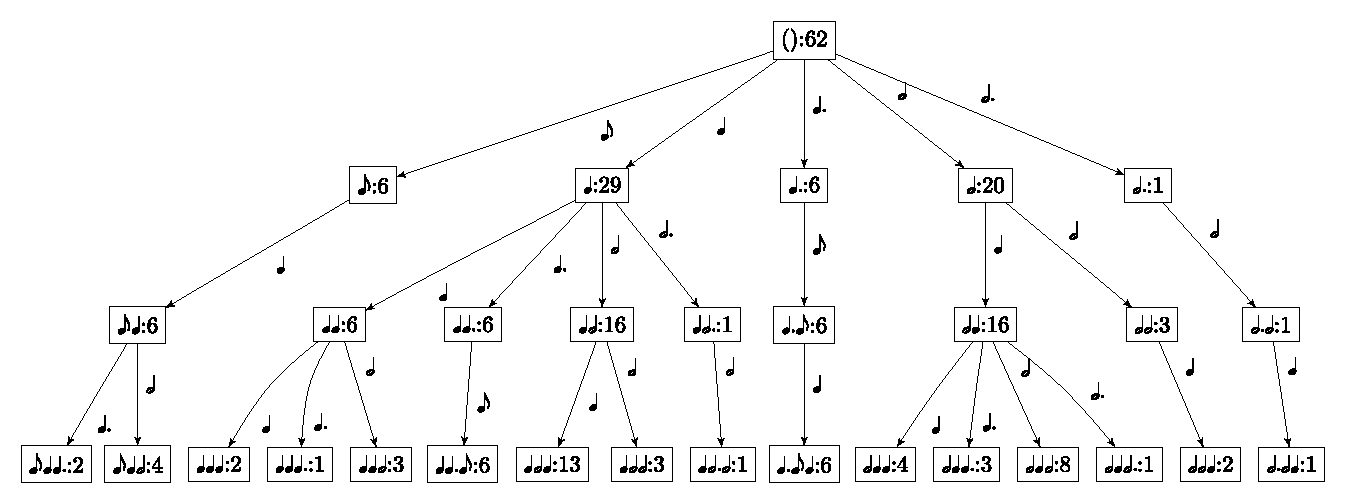
\includegraphics[width=455pt]{figs/duration_vp.pdf}
\caption{Trie for a context model over duration with $\hbar = 3$}
\label{fig:dur-trie}
\end{figure}

The algorithm for extracting $h$-grams for a training sequence $e_1^k$ works by
passing a sliding window of size $\hbar$ across the input sequence and
generating subsequences. This sliding window procedure is detailed in
Algorithm~\ref{alg:sliding-window} and illustrated in
Figure~\ref{fig:hgram-extract} for an input sequence $e_1^5$.

\begin{algorithm}[H]
  \caption{Sliding window algorithm for $h$-gram extraction}
  \label{alg:sliding-window}
  \begin{algorithmic}[1]
    \Function{learn-sequence}{$e_1^k \in [\tau]^*$}
      \For{$i : 1 \rightarrow k$}
        \State \Call{add-or-increment}{()}
        \For{$j : \min(1,i - \hbar) \rightarrow i$} \Call{add-or-increment}{$e_j^i$}
        \EndFor
      \EndFor
    \EndFunction
  \end{algorithmic}
\end{algorithm}

\begin{figure}[H]
\centering
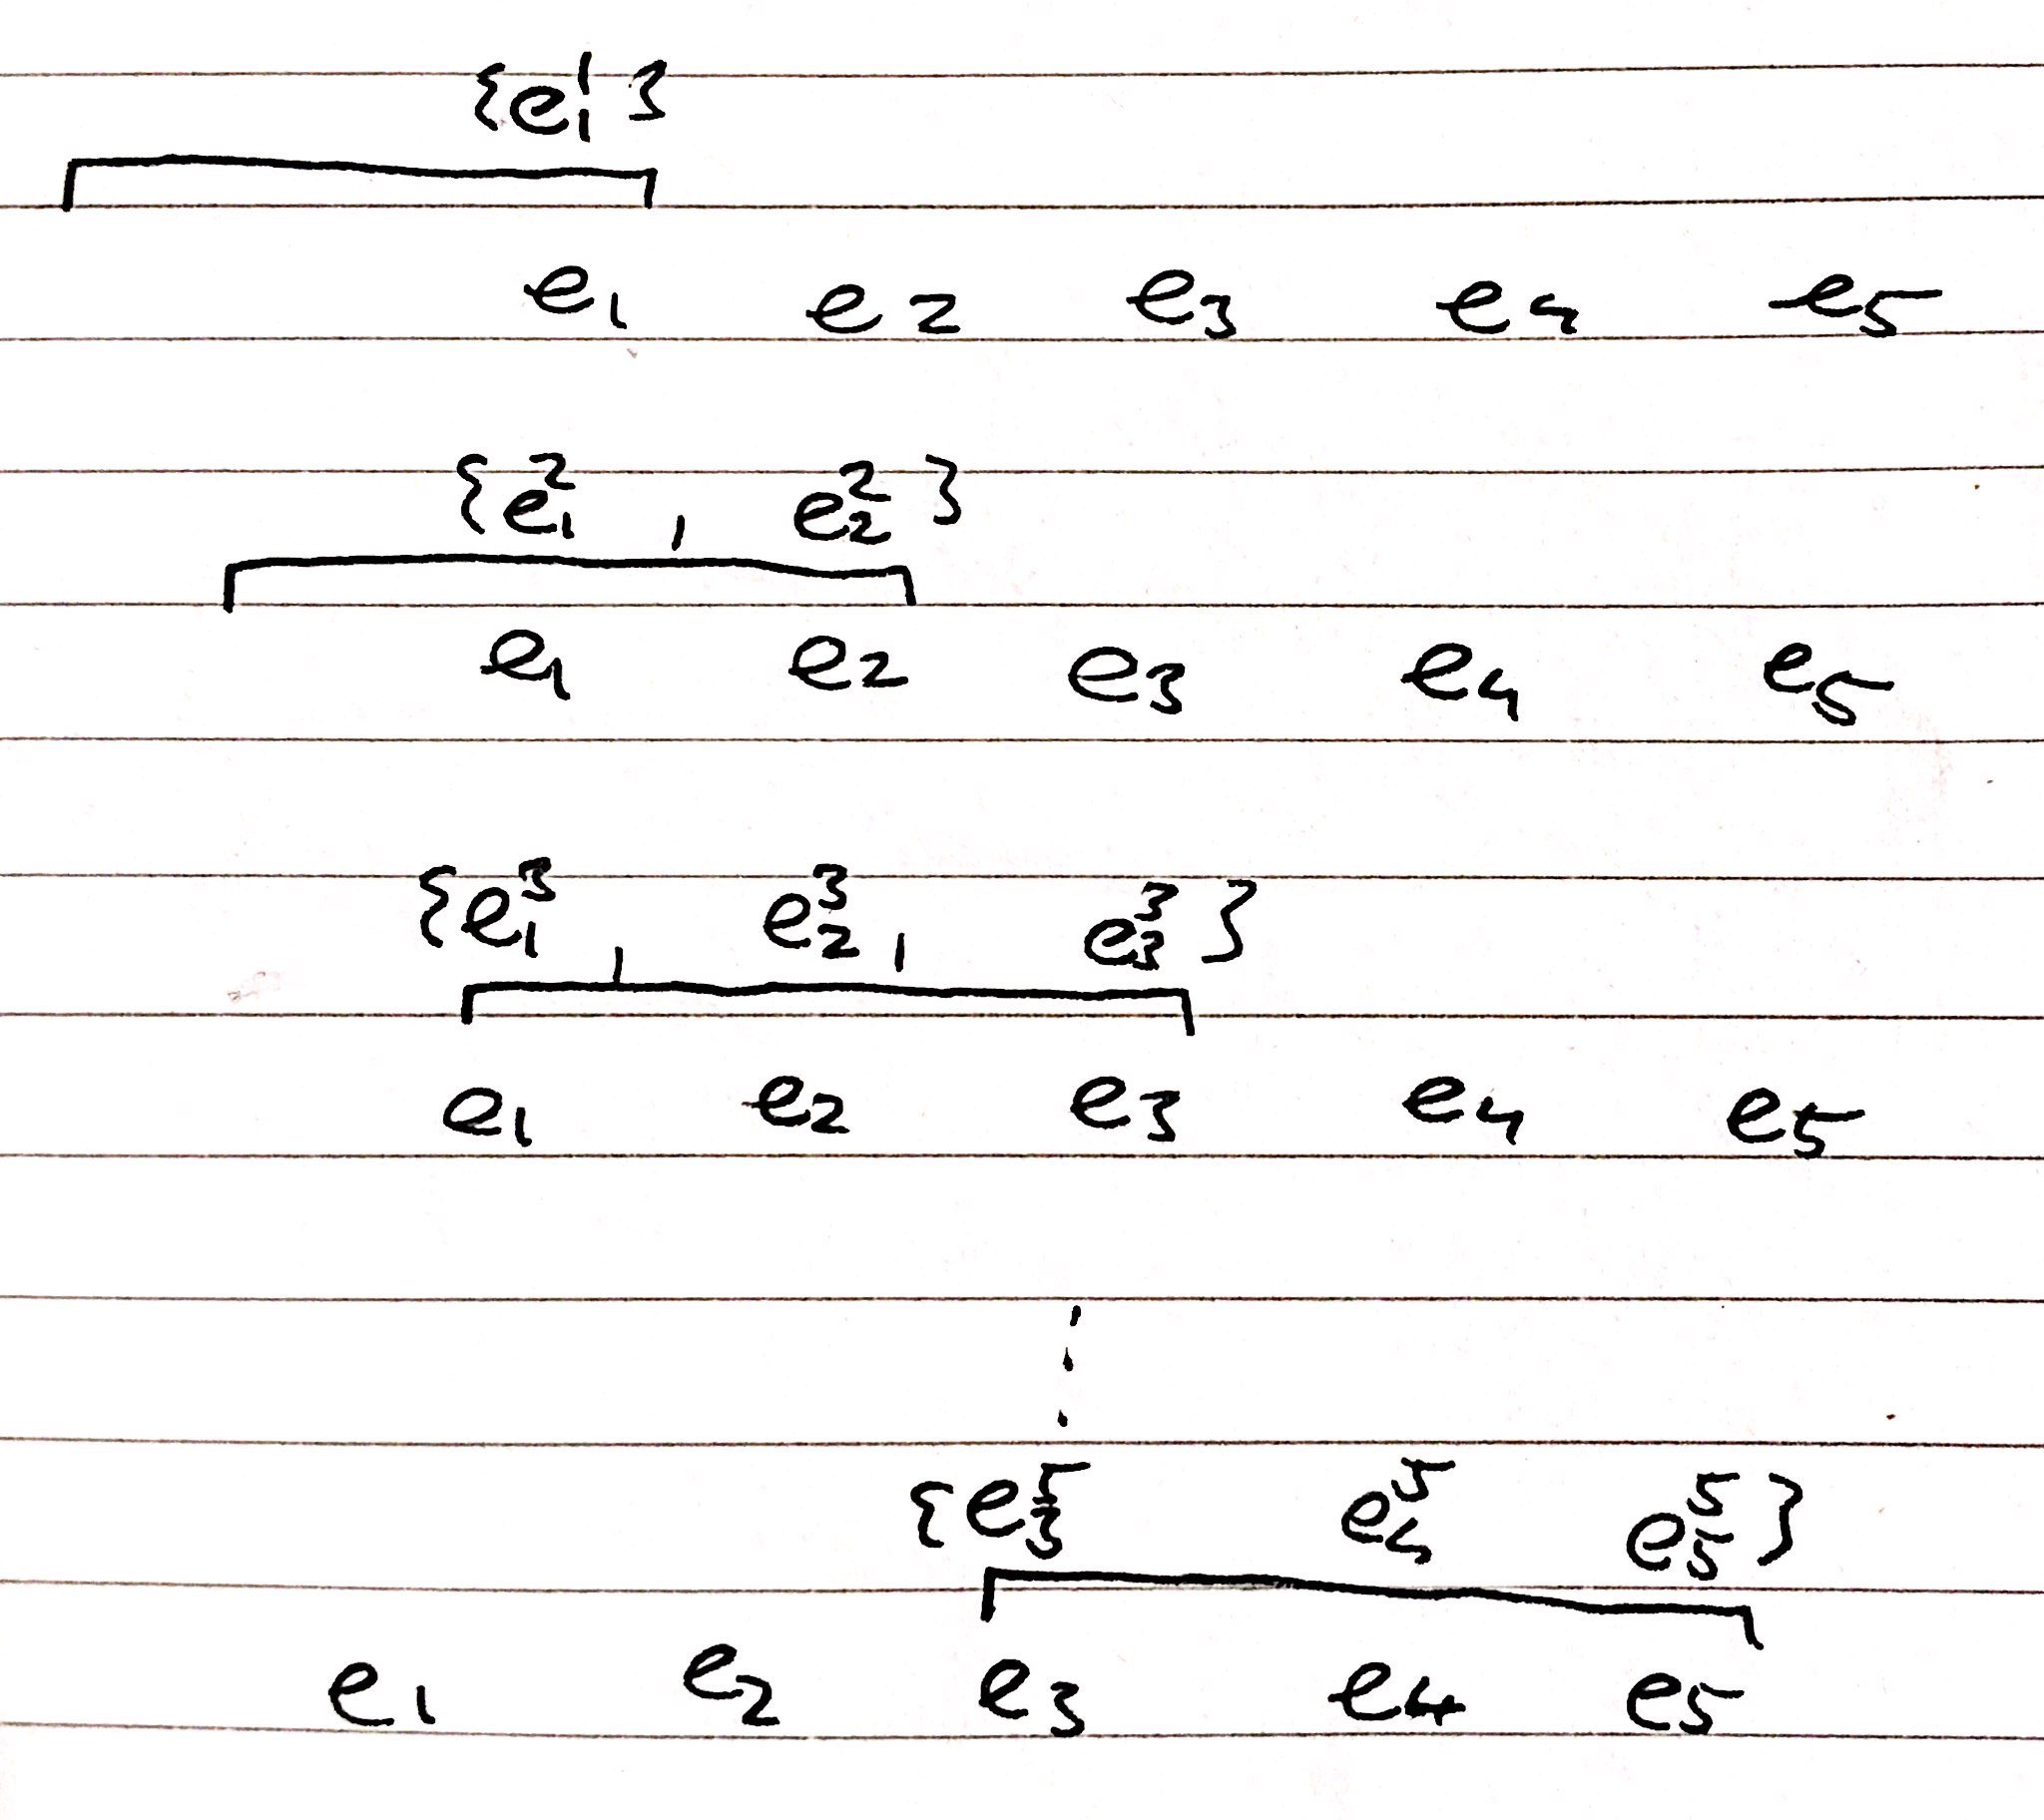
\includegraphics[width=300pt]{figs/sliding_window_tmp.jpg}
\caption{Illustration of the $h$-gram extraction algorithm with $\hbar = 3$}
\label{fig:hgram-extract}
\end{figure}

The subroutine \Call{add-or-increment}{$e_i^j$} looks up $e_i^j$ in the trie. If
it is found, then its count is incremented. Otherwise, $e_i^j$ is inserted into
the trie, the resulting node initialised with a count of unity. Note that $()$,
the empty sequence, corresponds to the root node in the trie.

Once we have constructed the trie for a context model, we need an algorithm to
perform \emph{inference}. In particular, we want to compute $\mathbb{P}(e' |
e_1^k)$ for some next event $e' \in [\tau]$ and input context $e_1^k \in
[\tau]^*$.

The maximum likelihood solution to this problem is simply to use the relative
frequency of the $h$-gram of interest:
\begin{equation}
  \mathbb{P}(e'|e_1^k) = \frac{ C(e_1^k::e') }{ \sum_{e''} C(e_1^k::e'') }
  \label{eq:ctx-max-like}
\end{equation}
where $C(e_i^j)$ denotes the count associated with $e_i^j$ in the trie, or $0$
if such a node does not exist. Note that all sequences longer than $\hbar$ (and
contexts longer than $\hbar-1$) are implicitly ignored, so $\forall j \in
\mathbb{N}.\ C(e_{k-\hbar-j}^k) = C(e_{k-\hbar+1}^k)$ and
$\mathbb{P}(e'|e_{k-\hbar+1-j}^k) = \mathbb{P}(e'|e_{k-\hbar+2}^k)$.

There are two main problems with this solution. The first is that we want our
models to be \emph{non-exclusive}; that is, $\forall e' \in [\tau].\
\mathbb{P}(e' | e_1^k) > 0$. An \emph{exclusive} model would limit the scope for
creativity in the system, and moreover, from a practical standpoint, evaluation
metrics such as \emph{cross-entropy} require calculating log-probabilities: we
therefore want to avoid zero probabilities. This model, however, fails to
guarantee non-exclusivity.

The second problem with this solution is that it does not deal with \emph{novel
contexts}. In particular, suppose we have not seen the context $e_1^k$. Then,
clearly, the denominator of (\ref{eq:ctx-max-like}) will be zero, which is
equally problematic.

An algorithm which attends to both of these issues is \emph{prediction by
partial match} (PPM) \cite{cleary1984ppm}. The central idea behind PPM is that,
instead of distributing the probability mass entirely among the exact context
matches, as per (\ref{eq:ctx-max-like}), we instead reserve some amount of the
probability mass known as the \emph{escape probability}. The escape probability
is then distributed recursively among a lower-order model. In this sense, PPM
is a form of \emph{backoff smoothing}.

Backoff smoothing algorithms are typically formulated recursively, as per
(\ref{eq:ppm-general}).
\begin{equation}\label{eq:ppm-general}
  \mathbb{P}(e' | e_1^k) = \begin{cases}
  \alpha(e'|e_1^k) & C(e' | e_1^k) > 0 \\
\gamma(e_1^k) \cdot \mathbb{P}(e' | e_{(k - \hbar) + 2}^k) & \text{otherwise}
\end{cases} 
\end{equation} 

If no match is found for any model, the recursion bottoms out with a uniform
distribution. The choice of \emph{escape probability} $\gamma(\cdot)$ is known
as the \emph{escape method}: established methods include A, B, C, D, and AX
\cite{pearce2004improved}. PPM A, the method implemented in this work, uses the
following $\alpha$ and $\gamma$ functions:
\begin{align}
  \label{eq:ppm-a}
  \alpha(e' | e_1^k) &= \frac{ C(e' | e_1^k) }{ 1 + \sum_{e''} C(e'' | e_1^k) }
  \\
  \gamma(e_1^k) &= \frac{ 1 }{ 1 + \sum_{e'} C(e' | e_1^k) }
  \label{eq:ppm-escape}
\end{align}

This recursive formulation can be somewhat misleading, as the notation implies
that (\ref{eq:ppm-general}) gives rise to properly normalised probability
distributions.  This is in fact not the case. Consider performing PPM with
$\hbar = 2$ over an alphabet $\Sigma = \set{\alpha,\beta,\gamma}$, and suppose
we learn the sequence $(\alpha,\beta,\gamma,\alpha,\alpha,\beta)$.
Figure~\ref{fig:bad-ppm-trie} illustrates the situation, and includes virtual
$\epsilon$-nodes to represent the escape mass.

\begin{figure}[H]
\centering
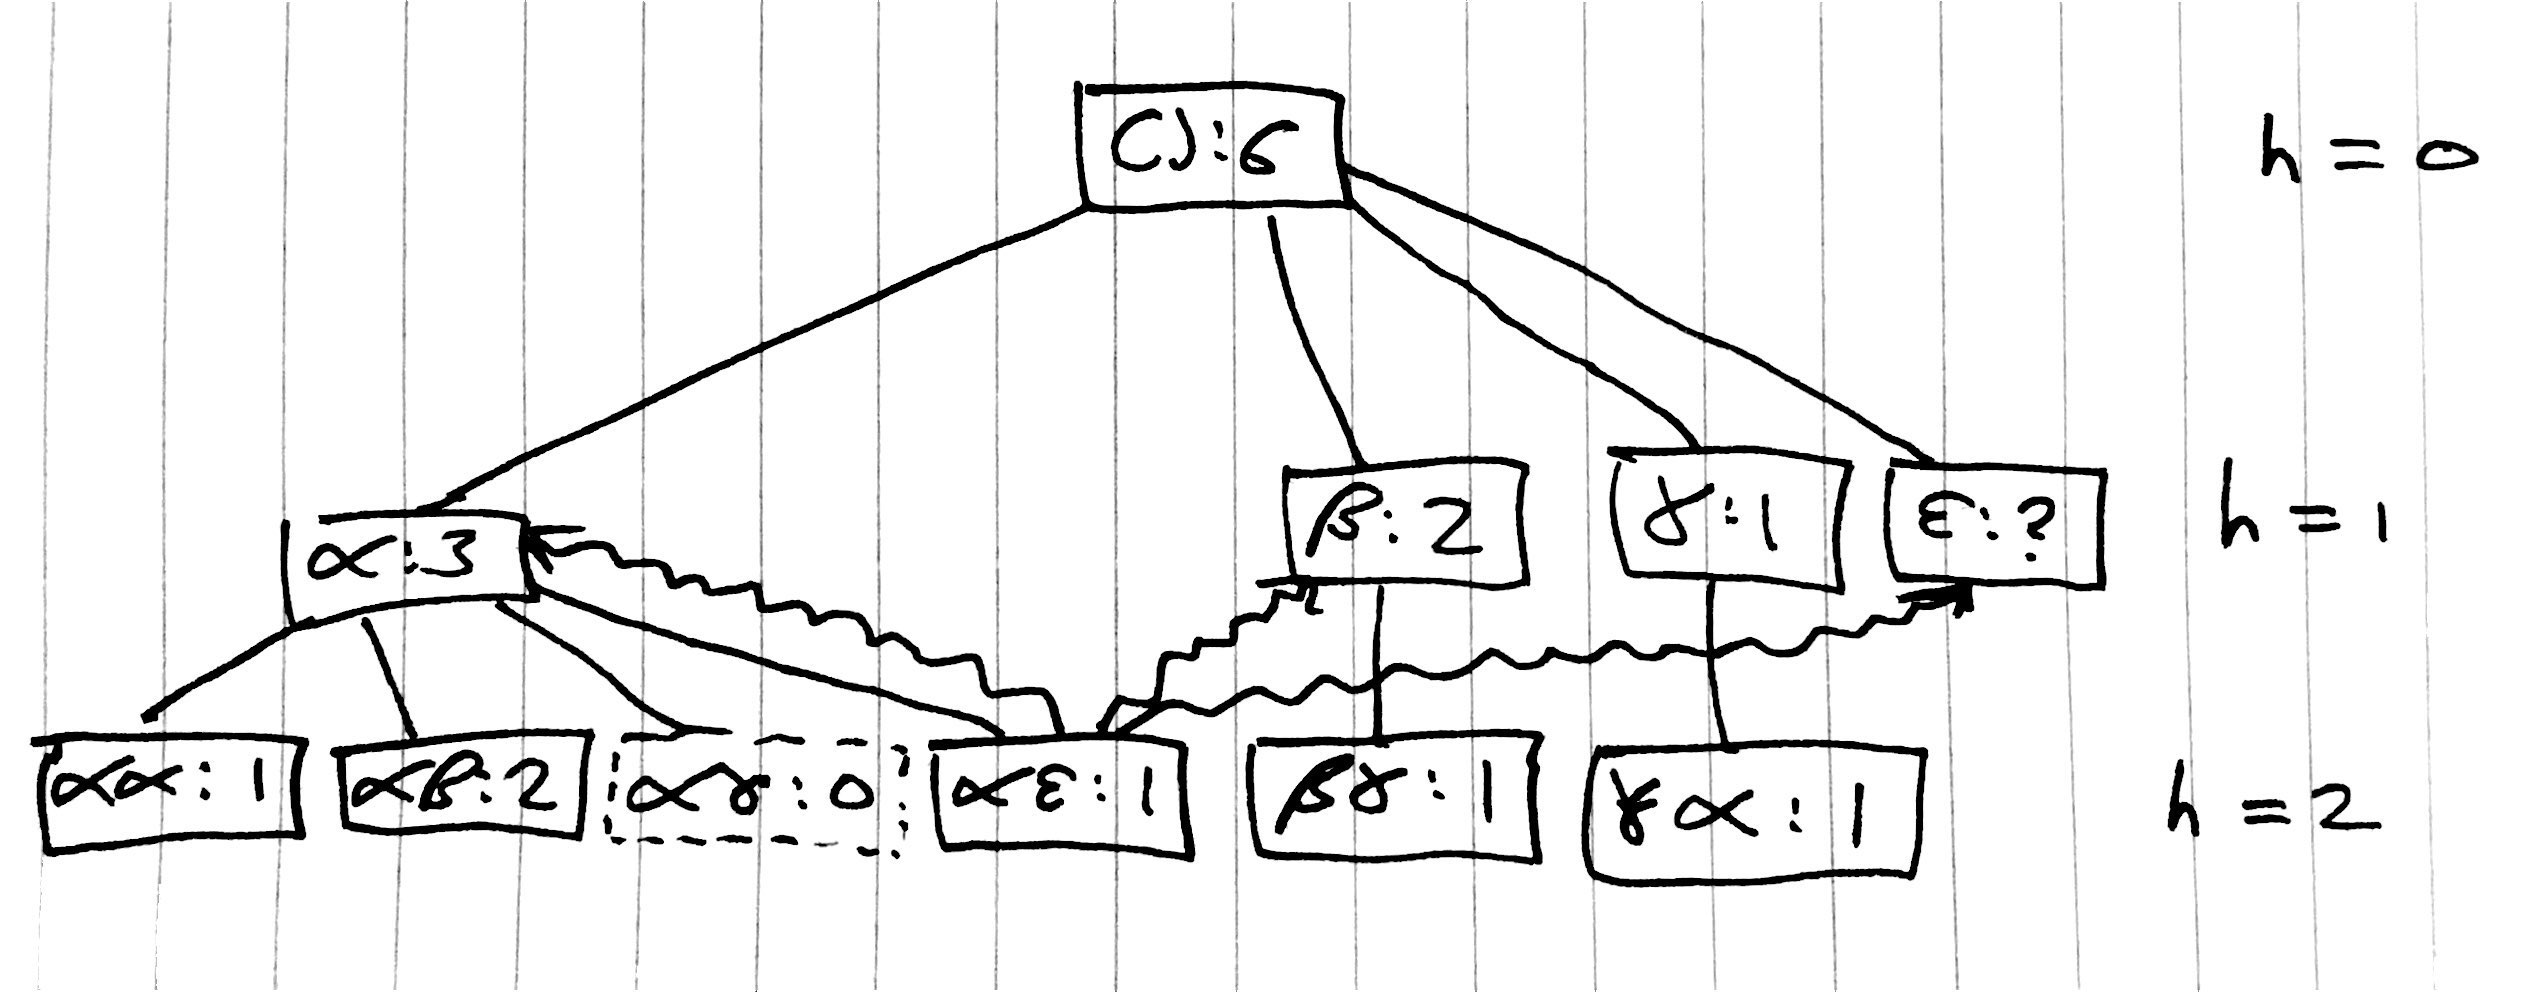
\includegraphics[width=400pt]{figs/problematic_trie_tmp.jpg}
\caption{Trie demonstrating lack of normalisation in standard PPM.}
\label{fig:bad-ppm-trie}
\end{figure}

The first problem is the escape node at layer $h = 1$. According to
(\ref{eq:ppm-escape}) it should have an effective count of $1$. However, this
yields:
$$ \sum_{e \in \Sigma} \mathbb{P}(e) = \frac{3}{7} + \frac{2}{7} + \frac{1}{7} =
\frac{6}{7} \neq 1. $$
The observation to make here is that if \emph{all} symbols in our alphabet have
a non-zero count for any given context, then the escape probability is
redundant. Suppose, then, we set the effective count of this $\epsilon$-node to
zero. Consider the distribution $\mathbb{P}(e|\alpha)$. We can trivially compute
$\mathbb{P}(\alpha|\alpha) = 1/4$ and $\mathbb{P}(\beta|\alpha) = 1/2$, and for
$\gamma$ we escape to find $\mathbb{P}(\gamma|\alpha) = 1/4 \cdot
\mathbb{P}(\gamma)$. However, $\mathbb{P}(\gamma) < 1$, so
$\mathbb{P}(e|\alpha)$ is not normalised. The problem here is that the escape
mass for the node labelled $\alpha\epsilon$ is distributed among all the symbols
at layer $h = 1$ in the trie, when in reality we can only ever escape to
$\gamma$.

There are two typical solutions for this lack of normalisation in PPM: in
earlier work, authors often simply compute an improper distribution and later
normalise it (e.g.\ \cite{conklin1990prediction}). A more sophisticated and less
wasteful solution which reasons about the possible $h$-grams that can be escaped
to is known as PPM with \emph{exclusion} \cite{pearce2004improved}, detailed in
Algorithm~\ref{alg:ppm-a}.

The key to exclusion in this algorithm is the \textit{Dead} set that is
maintained throughout the recursion. This set should be initialised to
$\varnothing$ and later populated with those events that we \emph{could} have
already matched at a higher-order model and therefore no longer need to consider
at lower-order models. To compute $\mathbb{P}(e' | e_1^k)$ we call
\Call{ppm-a}{$e_1^k$, $e'$, $1$, $\varnothing$}.

\begin{algorithm}[H]
  \caption{PPM A with exclusion}
  \label{alg:ppm-a}
  \begin{algorithmic}[1]
    \Function{ppm-a}{$e_1^k \in [\tau]^*$, $e' \in [\tau]$, $i_{\mathrm{begin}}$, 
    $\textit{Dead} \subseteq [\tau]$}
      \State $\textit{Alive} \gets [\tau] \setminus \textit{Dead}$
      \If{$i_{\mathrm{begin}} > k$}
      \State \Return $1 / |\textit{Alive}|$ \Comment{Base case: uniform
      distribution}
      \EndIf
      \State $i \gets i_{\mathrm{begin}}$
      \For{$i : i_{\mathrm{begin}} \rightarrow k$}
      \If{$C(e_i^k) > 0$} \textbf{break}
      \Comment{Find longest context match}
        \EndIf       
      \EndFor 
      \State $\textit{Known} \gets \set{ e'' \in [\tau]\ |\ C(e_i^k :: e'') > 0 }$
      \State $\textit{Novel} \gets Alive \setminus Known$ \Comment{All
      events we could escape for}
      \State $s \gets \sum_{e'' \in \textit{Alive}} C(e_i^k :: e'')$ 
      \If{$\textit{Novel} = \varnothing$}
        \State \Return $C(e_i^k :: e') / s$ \Comment{No possible need for escape}
      \EndIf
      \If{$e' \in \textit{Known}$}
      \State \Return $C(e_i^k::e') / (1 + s)$ \Comment{Matched $e_i^k::e'$}
      \EndIf
      \State \Return \Call{ppm-a}{$e_1^k$, $e'$, $i+1$, $Dead \cup Known$}$ / (1
      + s)$ \Comment{Escape recursively}
    \EndFunction
  \end{algorithmic}
\end{algorithm}

\subsection{Viewpoints}

One possible approach to modelling music would be to form a context model over
the entire event space $\zeta$.  Recall that $\zeta = [\tau_1] \times [\tau_2]
\times \cdots \times [\tau_n]$ is the cartesian product of many types. Aside
from being computationally expensive, this approach is severely limited in its
predictive power, since it requires an \emph{exact match} of the musical
context to make useful predictions: that is, there is no ability of the system
to \emph{generalise} to unseen contexts.

An obvious approach to allow the system to generalise would be to model some or
all of the $\tau_i$ \emph{independently}. To see why this might be useful,
consider that while there is certainly some correlation between e.g.\ pitch and
duration, much of the rhythmic regularity in a particular corpus is independent
of the pitch of the notes: thus, it is likely to be fruitful to model duration
independently of any of the other musical attributes.

Further, complex languages such as music can be viewed from many abstract
interpretations. One such abstract domain is the \emph{melodic
interval}: it is clear (\todo is it?) that intervalic patterns in music capture
regularity that is \emph{invariant} to the absolute pitch. To take this
abstraction to an extreme, we can consider the melodic \emph{contour}, which we
might represent with the domain $\set{-1,0,1}$, where the elements indicate a
decrease in pitch, stationary pitch, and increase in pitch respectively.
Modelling the regularity in such abstract domains and transforming the
predictions back into predictions over the concrete $\tau_i$ might therefore
further allow the system to generalise.  

\emph{Viewpoints} allow us to model music from these different points of view:
namely, we can model the individual $\tau_i$, as well as abstract
interpretations and combinations thereof. We now proceed to set up the formalism
of multiple viewpoints.

First, allow $\tau$ to range over types other than just the \emph{basic types}
that make up the component types of $\zeta$. We call these non-surface types
\emph{derived types}: the abstract interpretations derived from the surface
$\tau_i$. 

\textbf{Definition}. A \emph{viewpoint} modelling a type $\tau$ is:
\begin{enumerate}[label=\arabic*., itemsep=0mm]
  \item a partial function $\Psi_\tau : \zeta^* \rightharpoonup [\tau]$,
    together with
  \item a context model of sequences in $[\tau]^*$.
\end{enumerate}

The function $\Psi_\tau$ for a type $\tau$ is known as the \emph{projection}
function for $\tau$: it projects out the last element of type $\tau$ from some
surface event stream $e_1^k \in \zeta^*$, if such an element exists. Note that,
for convenience, we shall frequently refer to viewpoints simply by the type they
model. 

Viewpoints, as we have defined them, can clearly model individual surface and
derived types. While this is useful, we also want to be able to capture the
correlation between attributes.

\textbf{Definition}. A \emph{product type} $\tau_1 \otimes \cdots \otimes
\tau_n$ between $n$ types $\tau_1, \ldots, \tau_n$ is itself a type $\tau$ with
$[\tau] = [\tau_1] \times \cdots \times [\tau_n]$. 

For a product type $\tau = \tau_1 \otimes \cdots \otimes \tau_n$:
$$ \Psi_\tau(e_1^k) \triangleq
\begin{cases}
  \langle\Psi_{\tau_1}(e_1^k), \ldots, \Psi_{\tau_n}(e_1^k)\rangle & \forall i
  \in \set{1,\ldots,n}.\
  \Psi_{\tau_i}(e_1^k)\downarrow \\
  \bot & \text{otherwise.}
\end{cases}
$$

Viewpoints over product types are known as \emph{linked viewpoints}. 

Note that one can also make use of \emph{threaded viewpoints}: those defined
only at certain fixed intervals in a sequence. However, these are considered out
of scope for this work.

In order to train a viewpoint over type $\tau$, we need to provide the
underlying context model with sequences in $[\tau]^*$. To obtain such sequences
from surface events, we simply iterate the projection function $\Psi_\tau$ to
give a function $\Phi_\tau : \zeta^* \rightarrow [\tau]^*$ which we call the
\emph{lifting} function, defined as follows:
\begin{align*}
  \Phi_\tau(()) &\triangleq () \\
  \Phi_\tau(e_1^k) &\triangleq \begin{cases}
    \Phi_\tau(e_1^{k-1})::\Psi_\tau(e_1^k) & \Psi_\tau(e_1^k)\downarrow \\
    \Phi_\tau(e_1^{k-1}) & \text{otherwise.}
  \end{cases}
\end{align*}

In practice, we shall see that it is typically easier to implement $\Phi_\tau$
directly. However, formally, it is cleaner to specify $\Psi_\tau$ to define a
particular viewpoint.

Now consider a viewpoint over a type $\tau$ derived from some surface type
$\tau'$. This viewpoint will predict distributions over the abstract type
$\tau$, but we actually need a distribution over the concrete $\tau'$. 

The process of transforming a distribution from the abstract domain to the
concrete is given a limited treatment in the literature. Whorley
\cite{whorley2013phd} notes that this is effectively ``using the partial
function $\Psi_\tau$ in reverse on each of the viewpoint elements''. We argue
that the surface context is also needed to perform this task, and shall refer to
this process as \emph{reification}, specified by a partial function $\rho :
\zeta^* \times \mathrm{dist}(\tau) \rightharpoonup \mathrm{dist}(\tau')$, where
$\mathrm{dist}(\tau)$ denotes the set of probability distributions over a type
$\tau$. This shall be discussed further in Chapter~\ref{chap:impl}.

\subsection{Combining Viewpoint Predictions}\label{sec:vp-comb}

Recall that, given some musical context $e_1^k \in \zeta^*$, the goal is to
predict the next event $e_{k+1} \in \zeta$ where $\zeta = [\tau_1] \times \cdots
\times [\tau_n]$.  A collection of viewpoints that performs this task is known
as a \emph{multiple viewpoint system} (MVS). 

A MVS decomposes this task by predicting $e_{k+1}$ componentwise. Out of all the
viewpoints in the system, consider just those viewpoints capable of predicting
some $\tau_i$. At each timestep, given the context $e_1^k$, $N$ of these
viewpoints will \emph{activate}, meaning they predict a distribution for
$\tau_i$. This section concerns techniques for the combination of $N$ such
distributions to form an overall prediction. In particular, we consider
\emph{weighted} schemes as these are widely used in the literature and known to
perform better than unweighted schemes \cite{pearce2004combining}.

The premise of weighted schemes for viewpoint combination is that viewpoints
that are more `confident' in their predictions should be given higher weights.
Since the Shannon entropy of a viewpoint's distribution is a metric of overall
uncertainty, we use weights that are monotonically non-increasing as a function
of distribution entropy.

Suppose we have $N$ distributions over a type $\tau$. Suppose further that
there is some canonical ordering of $[\tau]$, such that we can pick out the
$j$\textsuperscript{th} member. Now, let $p_i(j)$ denote the probability
assigned to $j$ by the $i$\textsuperscript{th} of the $N$ distributions. We want
to combine these predictions to produce some overall distribution with
probabilities $p(j)$.

A general weighted arithmetic scheme combines the predictions as follows:
$$
  p(j) = \frac{ \sum_{i = 1}^N w_i p_i(j) }{ \sum_{i = 1}^N w_i }.
$$

\begin{figure}[H]
\centering
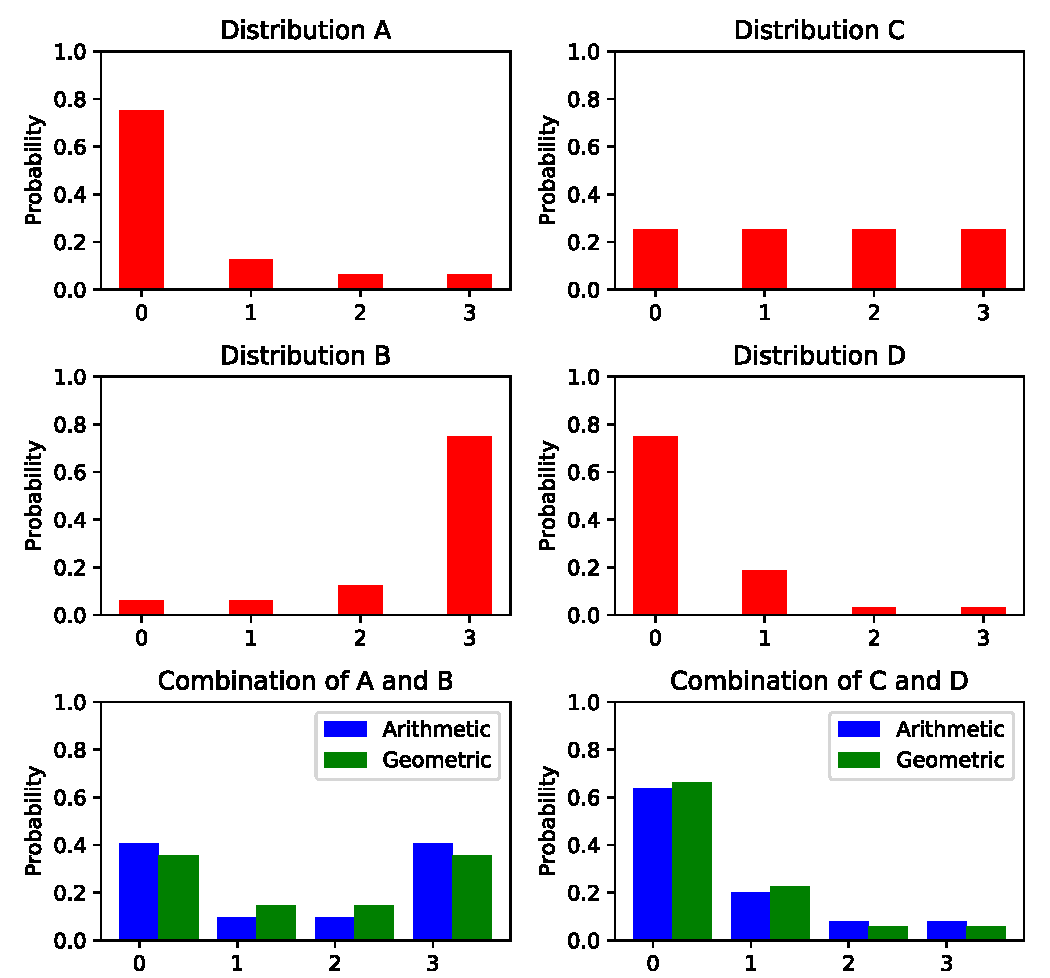
\includegraphics[width=400pt]{figs/dist_comb.pdf}
\caption{Plots illustrating effect of distribution combination schemes ($b = 2$)}
\label{fig:dist-comb-plot}
\end{figure}

The Shannon entropy of the $i$\textsuperscript{th} distribution is given by:
$$ H(i) = - \sum_{j = 1}^{|[\tau]|} p_i(j) \log_2 p_i(j) $$
with maximum value $H_{\mathrm{max}} = \log_2{ |[\tau]| }$. Now define the
\emph{normalised entropy} $\hat{H}(i)$ as:
$$ \hat{H}(i) \triangleq \begin{cases}
  H(i)/H_{\mathrm{max}} & H_{\mathrm{max}} > 0 \\
  1 & \text{otherwise.}
\end{cases} $$

In previous work this quantity has been called the \emph{relative entropy};
here, we use \emph{normalised entropy} so as to avoid confusion with the
Kullback-Leibler distance, which is also known by this name.

Finally, so that we can favour distributions with lower $\hat{H}$, we introduce
an exponential bias $b \in \mathbb{R}_0^+$:
$$ w_i = \hat{H}(i)^{-b}. $$

Note that we do not restrict $b$ to integer values, as is commonly done in the
literature \cite{whorley2013phd}. Pearce \cite{pearce2004improved} introduces a
new method for combining viewpoint predictions: namely, a \emph{weighted
geometric mean}:
$$ p(j) = \frac{1}{Z} \left( \prod_{i = 1}^N p_i(j)^{w_i} \right)^{ \frac{1}{
\sum_{i = 1}^N w_i }} $$

where $Z$ is a normalisation constant, and the $w_i$ are calculated as before.

Figure~\ref{fig:dist-comb-plot} shows the effect of using these two schemes on
some example distributions. It can be seen that a very low probability
prediction from one distribution has considerably more bearing with the
geometric scheme. Note also that when combining distributions $C$ and $D$, since
$D$ has much lower entropy, it has considerably more effect on the overall
result under both schemes.

\subsection{MVS Architecture}

\begin{figure}[H]
\centering
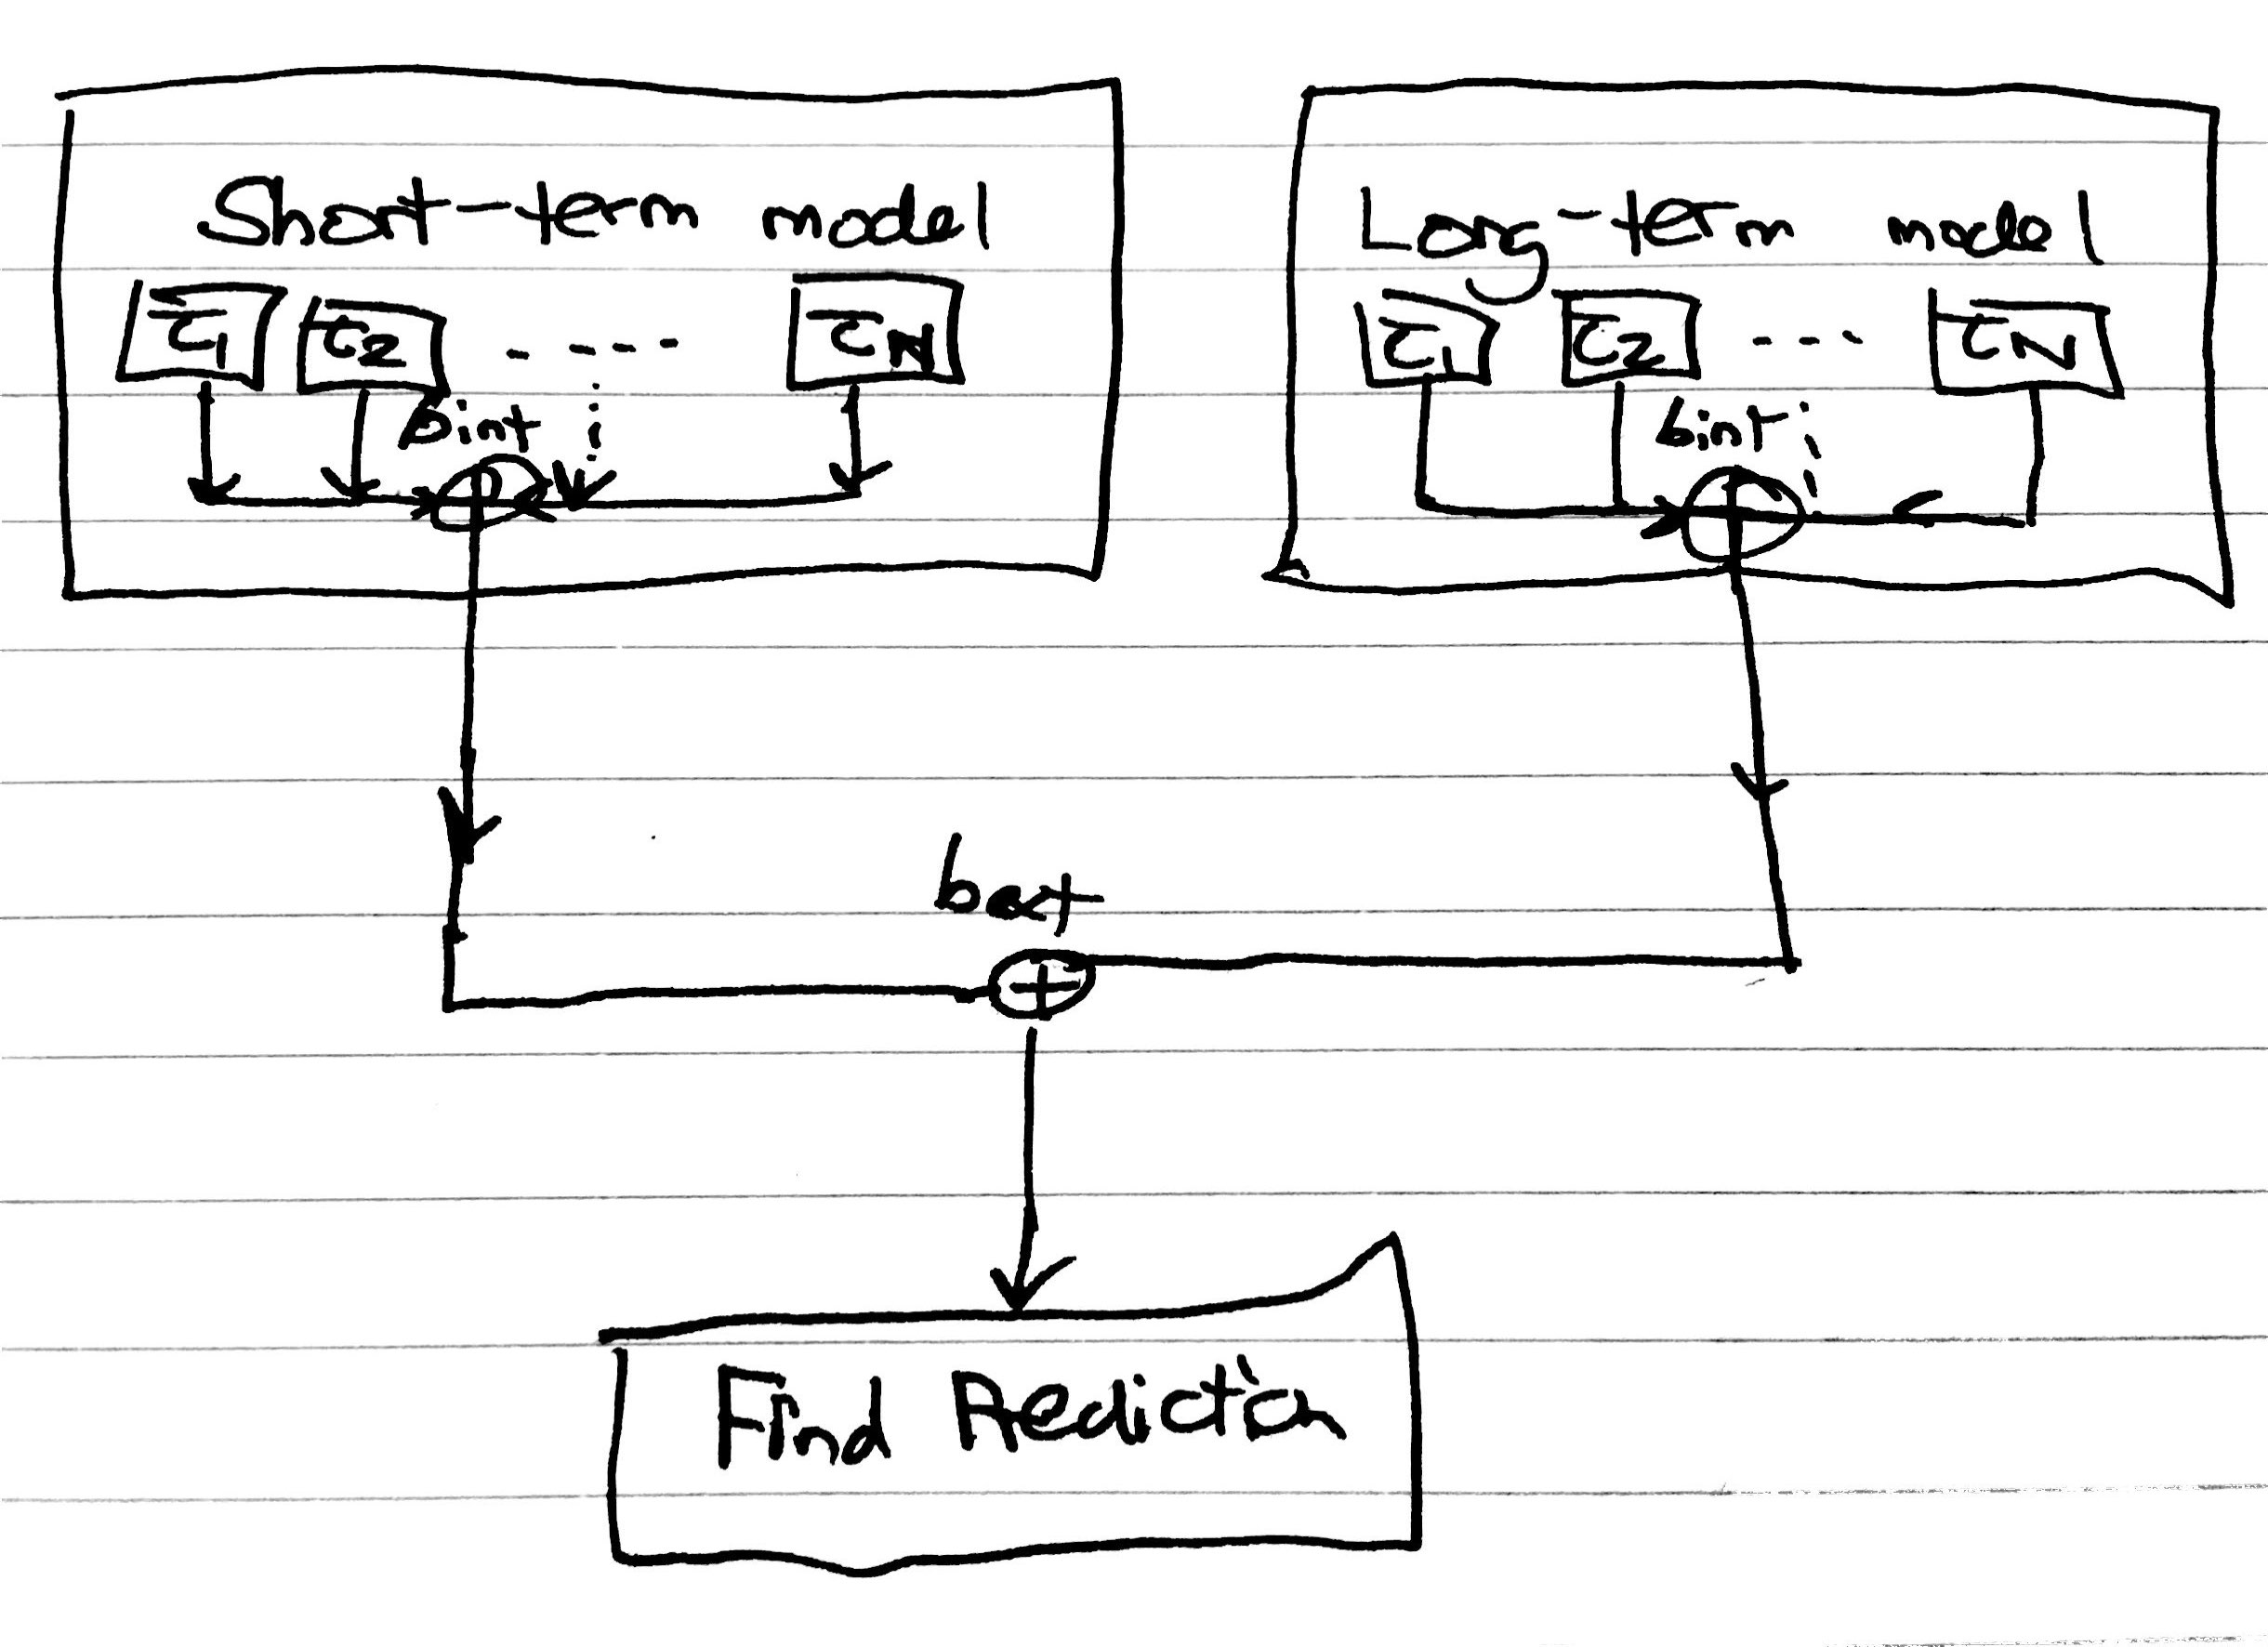
\includegraphics[width=250pt]{figs/mvs_arch_tmp.jpg}
\caption{Typical MVS architecture}
\label{fig:mvs-arch}
\end{figure}

For successful sequence prediction, it is necessary to capture both
intra-sequence and inter-sequence regularity: that is, the \emph{short-term}
effects \emph{local} to a particular sequence, and the \emph{long-term} effects
common through the entire corpus.  This is especially true of music, and the
chorales in particular, where entire melodic fragments are often re-used within
a given chorale melody.

In a conventional MVS architecture, this is achieved explicitly by using
entirely separate \emph{long-term} and \emph{short-term} models. The long-term
model is trained on the entire corpus, and the short-term model just on the
sequence being predicted or generated. Figure~\ref{fig:mvs-arch} illustrates
this architecture: viewpoint combination is indicated by $\oplus$, and is
performed as per Section~\ref{sec:vp-comb}.

In order to keep the number of hyperparameters under control, the following
architectural constraints are often enforced (and indeed, will be in this work):
\begin{itemize}
  \item The same set of viewpoints $\set{\tau_1, \ldots, \tau_N}$ is used in both
    the long-term and short-term model. 
  \item The viewpoints in the long-term model all have the same order bound
    $h_l$. Similarly, those in the short-term model all have a (possibly
    distinct) order bound $h_s$.
  \item The viewpoint combination within each of these two models is performed
    using the same bias parameter $b_{\mathrm{int}}$ and the combination of the
    short-term and long-term predictions using a separate bias parameter
    $b_{\mathrm{ext}}$.
\end{itemize}

\section{Recurrent Neural Networks}

\subsection{Basic RNN}

\todo RNN explanation with diagram as per Goodfellow DL book.

\subsection{LSTM}

\todo Explain exploding/vanishing gradients.

\todo LSTM explanation, citing papers on constant gradient flow.

\subsection{Regularisation}

\todo Explain dropout applied to RNN.

\subsection{Tooling}

\todo Explain TensorFlow, \textbf{why it was chosen}, notion of computational
graph, etc.

\chapter{Implementation}\label{chap:impl}

\section{Corpus Preparation and Analysis}

\todo Maybe some graphs illustrating distributions in corpus as per
\texttt{analyse\_corpus.py}.

\section{Multiple Viewpoint System}

\todo Using the framework of multiple viewpoints outlined in the preparation,
discuss the \emph{specific} viewpoints implemented.

\subsection{Software Architecture}

\todo Diagram illustrating the (code) architecture of the MVS. 

\todo Explain use of
\texttt{C++} templates illustrating correspondence between formalism and
implementation.

\subsection{Unit Tests}

\todo Get lots of points and stickers for demonstrating good software
engineering practice by testing thoroughly.

\section{Recurrent Neural Network}

\subsection{Early Experiments}

\todo Mention language modelling precursor: maybe include snippet of output?

\subsection{Corpus Preprocessing}

\todo Describe the method of \emph{tonal inflation} in order for the RNN to
learn the key as an emergent property of each composition.

\subsection{Domain-specific Features}

\todo Explain ``clock'' inputs. Discuss symmetry with multiple viewpoints.

\chapter{Evaluation}\label{chap:eval}


\chapter{Conclusion}

\todo Write me.

%%%%%%%%%%%%%%%%%%%%%%%%%%%%%%%%%%%%%%%%%%%%%%%%%%%%%%%%%%%%%%%%%%%%%
% the bibliography
\phantomsection
\printbibliography
\addcontentsline{toc}{chapter}{Bibliography}
\todo Check all the references for typos as Google Scholar certainly has a few!

%%%%%%%%%%%%%%%%%%%%%%%%%%%%%%%%%%%%%%%%%%%%%%%%%%%%%%%%%%%%%%%%%%%%%
% the appendices
\appendix

\chapter{Project Proposal}

\todo uncomment me!
%% Note: this file can be compiled on its own, but is also included by
% diss.tex (using the docmute.sty package to ignore the preamble)
\documentclass[12pt,a4paper,twoside]{article}
\usepackage[UKenglish]{isodate}
\usepackage[pdfborder={0 0 0}]{hyperref}
\usepackage[margin=25mm]{geometry}
\usepackage{graphicx}
\usepackage{parskip}
\usepackage{enumitem}
% \usepackage{mathpazo}
% \usepackage{eulervm}
\usepackage{microtype}

\usepackage[style=numeric,backend=bibtex]{biblatex}
\bibliography{refs.bib}

\begin{document}

\cleanlookdateon

\begin{center}
\Large
Computer Science Tripos -- Part II -- Project Proposal\\[4mm]
\LARGE
A Comparison of Statistical Models and Recurrent Neural Networks Applied to the
Generation of Music\\[4mm]

\large
Alex Coplan, St Catharine's College

Originator: Alex Coplan

\today
\end{center}

\vspace{5mm}

\textbf{Project Supervisor:} Matthew Ireland

\textbf{Director of Studies:} Dr S. Taraskin

\textbf{Project Overseers:} Dr M. Fiore \& Dr I. Leslie

% Main document

\section*{Introduction}

The goal of this project is to implement, evaluate, and compare two different
techniques for the algorithmic generation of music. I am particularly interested
in the generation of melody, and ultimately, \emph{polyphony}: multiple
independent melodies interacting with each other in harmonic coherence. In
particular, the two classes of techniques I intend to consider for this project
are:
\begin{itemize}[itemsep=0mm]
	\item Statistical history models such as \emph{multiple viewpoint
			systems} \cite{conklin1995viewpoints}.
	\item Recurrent neural networks.
\end{itemize}

The exact statistical model(s) to be investigated will be determined by the end
of the research phase of the project.

Algorithmic composition is of general interest in computational creativity, but
also has a number of practical applications; one such application being in
\emph{machine-assisted composition}, where a music generation tool aids a human
composer by extending or generating musical ideas. Such tools would be used by a
wide variety of music practitioners.

My intention is to undertake an investigation into the algorithmic composition
of polyphonic music. The first major problem that needs to be tackled in such an
endeavour is that of melody generation. Once this problem has been addressed,
one would subsequently consider the problem ``given a melody (the
\emph{subject}), compose a second (independent) melody (the
\emph{countersubject}) which interacts with, and is coherent with the subject.''
Since the lines in polyphony should be \emph{independent} melodies, it is
necessary to approach the problem of melody generation first.

I therefore propose that the core of the project investigate the application of
these techniques to melody generation. As an optional extension, an
investigation could then be carried out into the composition of two-part
polyphonic music, using these techniques and/or extensions thereof.

I shall follow the approach often taken in the literature of restricting the
domain of source material to stem from a particular musical idiom, e.g.\
\cite{pearce2001evaluation}. This is desirable for a number of reasons, not
least because it introduces a useful evaluation criterion: do the compositions
produced by the system exhibit a coherent musical style, consistent with that
exhibited by the material in the corpus?

In order for this project to be evaluated effectively, in addition to any
information-theoretic or music-theoretic analyses, it is necessary to perform
listening trials on human subjects. Pearce et al.\ \cite{pearce2001evaluation}
outline a framework for evaluation which allows more scientific claims to be
made as a result of the evaluation process. Evaluation would be performed in the
form of a blind trial where the subjects are asked to classify compositions as
human or machine-composed. In this work, it is noted that the participants
exhibited a bias towards classifying compositions as machine composed. This is
something that should be taken into account when designing the evaluation
methodology. An avenue for investigation in this respect is the method of
\emph{three-alternative forced choice}.

Conklin \cite{conklin2003music} notes that random walk is not necessarily the
best method of sampling from a statistical distribution such as that of a
multiple viewpoint system or Markov chain. In this project, I would therefore
also consider exploring different techniques for sampling from statistical
models.
 
\subsection*{Background}

Markov processes are natural statistical models for the analysis of melody, and
are well known as tools for composition \cite{ames1989markov}. Although
effective, Markov processes are far from perfect tools for modelling music.
Specifically, a basic pitch-duration Markov process disregards a considerable
amount of musical information available in the context
\cite{conklin1995viewpoints}.  

However, simply incorporating more musical features into the state space of a
Markov chain leads to an exponential blow-up in space complexity and
necessitates both a large amount of training data for good performance, as well
as solving the sparse data problem (\cite{conklin2003music}, section 2.1).
Moreover, Markov chains do not make use of the long-term context of a system,
which is necessary for modelling the broader sense of sequence and structure
which is present in music.

Conklin et al.\ \cite{conklin1995viewpoints} introduce the method of
\emph{multiple viewpoints} which uses the interpolation of the predictions of
many different context models, each of which considers a different musical
attribute (or some combination of attributes). These include both short-term and
long-term attributes, enabling this method to capture sequence and structure.

It is well known that Recurrent Neural Networks (RNNs) can effectively generate
sequences. RNNs have seen more successful application in music following the
introduction of long short-term memory (LSTM) techniques \cite{eck2002lstm}.
Without use of LSTM, RNNs exhibit similar problems to Markov chains in that the
output does not contain the elements of sequence and structure that one might
expect from compositions in the corpus.

\section*{Starting point}

In Lent term of 2016, I gave a talk (as part of Churchill college's Computer
Science talk series) on melody generation using Markov chains. I also
constructed a demo in Ruby which implemented a parser for ABC
notation\footnote{\url{http://abcnotation.com/}} along with a simple Markov
chain model, trained of a small corpus of hymn tunes, which generated tunes by
random walk. 

Although this experience led me to this choice of project, the implementation of
a model such as a multiple viewpoint system is considerably more involved, and
the architecture vastly different. The implementation of this model will
therefore be carried out from scratch.  The neural network will be implemented
using a library such as Google's
TensorFlow\footnote{\url{https://www.tensorflow.org/}}.

As an organ scholar (and previously an A-Level music student), I have
considerable experience with performing polyphonic music (and some experience of
analysis), especially that of the renaissance and baroque eras. I believe this
domain knowledge will prove especially useful for making musically-informed
decisions in this project. 

\section*{Resources required}

For this project I shall primarily use my own laptop. Backup will be primarily
in the form of a GitHub-hosted repository, but I will also perform backups of
the project files to an external hard drive as well as multiple cloud providers
(Google, Apple, Dropbox) and the MCS. Should my main computer suddenly fail, I
can easily continue the project using MCS computers by cloning the code from the
GitHub repository.

Although datasets can easily be compiled from online sources, it may also be of
use to have a MIDI keyboard to be able to input arbitrary musical data. I own a
MIDI keyboard which would be suitable for these purposes. I will make use of
open-source software (such as MuseScore\footnote{\url{https://musescore.org/}})
for synthesis of MIDI and other musical data. I require no other special
resources.

\section*{Work to be done}

I will employ an agile software development methodology when undertaking this
project. The ordered list of sub-tasks within this project are:
\begin{enumerate}

\item Devising and implementing an internal representation of musical data,
	along with a simple ``music theory engine'' to process this data.  

\item Implementing a simple parser for some form of input notation (ABC, MIDI,
	MusicXML); the exact form to be determined in the research phase.  

\item Implementing and iteratively refining the statistical model (e.g. multiple
	viewpoint system).

\item Implementing and iteratively refining the RNN for melody generation.  

\item Designing and carrying out a scheme for human evaluation.

\item Making iterative improvements to the two models.

\end{enumerate}

\section*{Success criteria}

\subsection*{Core Tasks}

The project will be a success if I have:
\begin{itemize}
	\item Successfully implemented a statistical model such as a multiple
		viewpoint system capable of generating melody.
	\item Successfully implemented a technique based on recurrent neural
		networks capable of generating melody.
	\item Performed an evaluation and comparison of the two
		models, answering questions such as:
	\begin{itemize}
		\item Can human subjects distinguish the machine-composed output
			from the human-composed samples in the corpus?
		\item Do human subjects classify the machine-composed output as
			adhering to the specified style?
	\end{itemize}

	Note that the success of the evaluation stage is not predicated on the
	answers to the questions given above, but merely whether the evaluation
	is conducted in a scientific manner.
\end{itemize}

\subsection*{Extension Tasks}

The project will be judged as a success if all the core tasks have been
completed. The extension tasks won't be used to judge the success of the
project, but it will have gone above and beyond expectations if one of them is
completed.

These possible extensions include:
\begin{itemize}
	\item Extending a multiple viewpoint system to generate polyphony.
	\item Extending a RNN to generate polyphony.
	\item Exploring extensions and adaptations of multiple viewpoint
		systems.
\end{itemize}

\section*{Timetable}

Planned starting date is 16/10/2011.

\begin{tabular}{ p{4cm} | p{11cm} } \hline 
% TODO: 2 week blocks, start earlier to include proposal week.
% TODO: 2-page spread

16/10/16 - 27/10/16 Mich. Weeks 2-4 & \textbf{Research phase}.
Research multiple viewpoint systems, RNNs, and evaluation techniques.
Investigate options for corpus material and format. This will inform the type of
parser that should subsequently be implemented. Devise and fix an internal
representation for musical data. Design specific multiple viewpoint system based
on \cite{whorley2013phd}. The corpus should also be prepared as fully as
possible during this stage. Familiarisation with libraries (e.g. TensorFlow)
should be accomplished during this phase.

\textbf{Milestone}: Report summarising research handed to supervisor.
\\ \hline
03/11/16 - 10/11/16 \newline Mich. Week 5 & \textbf{Preliminary Implementation}. 
Implement parser for chosen corpus format. Implement internal representation as
determined in the previous phase. Write test suite for the above. 
\\ \hline
10/11/16 - 30/11/16 \newline Mich. Weeks 6-8 & \textbf{MVS Implementation I}.
First iteration of multiple viewpoint system to be completed in these three
weeks. System need not be complete in terms of the exact viewpoints used.
However, the underlying machinery should be. In particular, context models,
viewpoint representation, prediction interpolation etc. should all be
implemented, such that a MVS can be constructed, trained, and used for
generation.
\\ \hline
01/12/16 - 22/12/16 \newline Christmas Vac. Weeks 1-3 & \textbf{RNN Implementation I}.
Implement LSTM Recurrent Neural Network. 
\\ \hline
29/12/16 - 12/01/17 \newline Christmas Vac. Weeks 4-5 & \textbf{MVS Implementation II}.
Implement full multiple viewpoint system. Investigate different choices of
viewpoints as per the R\&D outlined in the research phase. 
\\ \hline
12/01/17 - 26/01/17 \newline Lent Week 0 & \textbf{RNN Implementation II}.
Finish RNN implementation. Train network on entire corpus.
\\ \hline

\end{tabular}

\printbibliography

\end{document}


\end{document}
